%%% Econ714: Macroeconomics II
%%% Spring 2021
%%% Danny Edgel
%%%
% Due on Canvas Monday, February 1st, 11:59pm Central Time
%%%

%%%
%							PREAMBLE
%%%

\documentclass{article}

%%% declare packages
\usepackage{amsmath}
\usepackage{amssymb}
\usepackage{array}
\usepackage{bm}
\usepackage{changepage}
\usepackage{centernot}
\usepackage{graphicx}
\usepackage[shortlabels]{enumitem}
\usepackage{fancyhdr}
	\fancyhf{} % sets both header and footer to nothing
	\renewcommand{\headrulewidth}{0pt}
    \rfoot{Edgel, \thepage}
    \pagestyle{fancy}
	
%%% define shortcuts for set notation
\newcommand{\Z}{\mathbb{Z}}
\newcommand{\R}{\mathbb{R}}
\newcommand{\Q}{\mathbb{Q}}
\newcommand{\lmt}{\underset{x\rightarrow\infty}{\text{lim }}}
\newcommand{\neglmt}{\underset{x\rightarrow-\infty}{\text{lim }}}
\newcommand{\zerolmt}{\underset{x\rightarrow 0}{\text{lim }}}
\newcommand{\loge}[1]{\text{log}\left(#1\right)}
\newcommand{\usmax}[1]{\underset{#1}{\text{max }}}
\newcommand{\Mt}{M_{t+1}^t}
\newcommand{\vhat}{\hat{v}}
\newcommand{\olp}{\overline{p}}
\renewcommand{\L}{\mathcal{L}}
\newcommand{\olq}{\overline{q}}
\newcommand{\zinf}{_{t=0}^\infty}
\newcommand{\aneg}{A^{-1}}
\newcommand{\sneg}{s^{-1}}
\newcommand{\olk}{\overline{k}}
\newcommand{\olc}{\overline{c}}
\newcommand{\olr}{\overline{r}}
\newcommand{\olpi}{\overline{\pi}}
\newcommand{\Aneg}{A^{-1}}
\renewcommand{\sneg}{s^{-1}}
\newcommand{\dc}[1]{\Delta c_{#1}}
\newcommand{\N}{\mathcal{N}}

\newcommand{\E}[1]{\mathbb{E}\left[#1\right]} % expected value
\newcommand{\Et}[1]{\mathbb{E}_t\left[#1\right]}

%%% define column vector command (from Michael Nattinger)
\newcount\colveccount
\newcommand*\colvec[1]{
        \global\colveccount#1
        \begin{pmatrix}
        \colvecnext
}
\def\colvecnext#1{
        #1
        \global\advance\colveccount-1
        \ifnum\colveccount>0
                \\
                \expandafter\colvecnext
        \else
                \end{pmatrix}
        \fi
}

%%% define function for drawing matrix augmentation lines
\newcommand\aug{\fboxsep=-\fboxrule\!\!\!\fbox{\strut}\!\!\!}

\makeatletter
\let\amsmath@bigm\bigm

\renewcommand{\bigm}[1]{%
  \ifcsname fenced@\string#1\endcsname
    \expandafter\@firstoftwo
  \else
    \expandafter\@secondoftwo
  \fi
  {\expandafter\amsmath@bigm\csname fenced@\string#1\endcsname}%
  {\amsmath@bigm#1}%
}


%________________________________________________________________%

\begin{document}

\title{	Problem Set \#1 }
\author{ 	Danny Edgel 					\\ 
			Econ 714: Macroeconomics II		\\
			Spring 2021						\\
		}
\maketitle\thispagestyle{empty}

%%%________________________________________________________________%%%

\noindent\textit{Collaborated with Sarah Bass, Emily Case, Michael Nattinger, and Alex Von Hafften}

%%%________________________________________________________________%%%

\subsection*{Question 1}

The social planner's problem is:
\[
	\usmax{\{I_t,C_t,K_{t+1}\}_{t=0}^\infty}\beta^tU(C_t)\text{ s.t. }K_{t+1} = (1-\delta)K_t + I_t - D_t\text{, } C_t + I_t\leq F(K_t)
\]
At any optimum, the resource constraint will hold with equality, so we can combine the law of motion and the resource constraint to obtain a single constraint:
\[
	F(K_t) = K_{t+1} - (1-\delta)K_t + C_t + D_t 
\]
We can derive the Euler equation by taking the first-order conditions of the Lagrangian function.:
\[
	\L = \sum_{t=0}^\infty \beta^tU(C_t) - \lambda_t\left(F(K_t) - K_{t+1} + (1-\delta)K_t - C_t - D_t \right)
\]
\begin{align*}
	\frac{\partial \L}{\partial C_t} 		= \beta^tU'(C_t)+\lambda_t 										&= 0	\\
	\frac{\partial \L}{\partial K_{t+1}}	= \lambda_t - \lambda_{t+1}\left(F'(K_{t+1}) + 1-\delta\right) 	&= 0	
\end{align*}
Taken together, these first-order conditions give us the Euler equation for the SPP:
\[
	U'(C_t) = \beta U'(C_{t+1})\left[F'(K_{t+1})+1-\delta\right]
\]


%%%________________________________________________________________%%%
\pagebreak
\subsection*{Question 2}
Given the steady-state value $D$, the steady-state values of capital, ${K_t=K_{t+1}=\overline{K}(D)}$, and consumption, ${C_t=C_{t+1}=\overline{C}(D)}$ are detemined by the intersection of the resource constraint and Euler equation when capital and consumption are held constant:
\begin{align*}
	U'(\overline{C}) = \beta U'(\overline{C})\left[F'(\overline{K})+1-\delta\right] 
		&\Rightarrow \beta\left[F'(\overline{K})+1-\delta\right] = 1	\\
	F(\overline{K}) = \overline{K} - (1-\delta)\overline{K} + \overline{C} + D
		&\Rightarrow F(\overline{K}) = \delta\overline{K} + \overline{C} + D
\end{align*}
The phase diagram for the solution is displayed below, with the three steady states marked by blue dots.
\begin{center}
	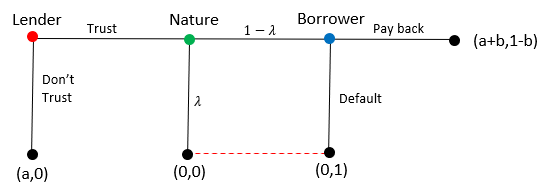
\includegraphics[scale=.6]{figure1.png}
\end{center}

%%%________________________________________________________________%%%

\subsection*{Question 3}

\begin{center}
	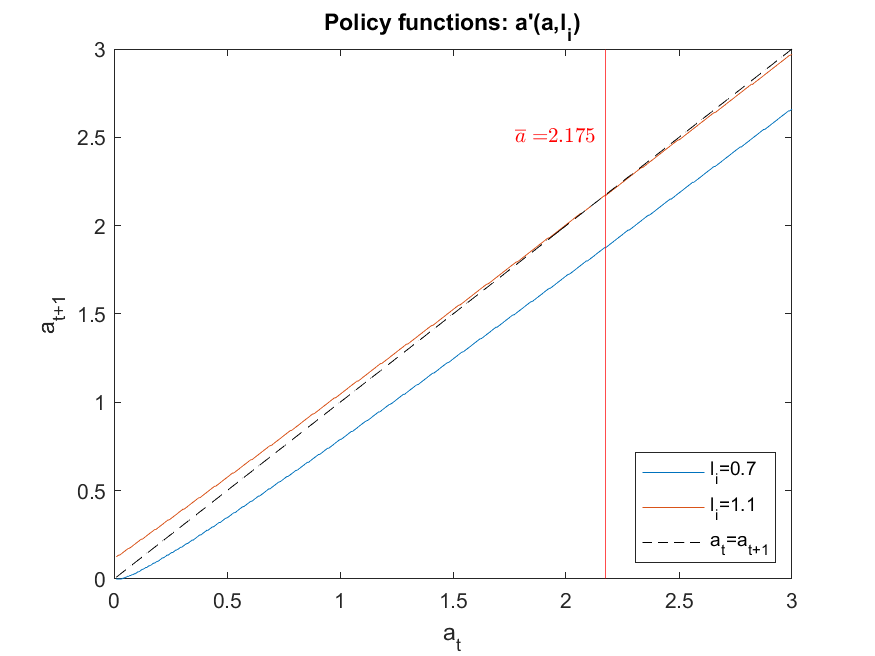
\includegraphics[scale=.6]{figure2.png}
\end{center}

%%%________________________________________________________________%%%

\subsection*{Question 4}

\begin{center}
	\includegraphics[scale=.7]{figure4a.png} \includegraphics[scale=.7]{figure4b.png}
\end{center}

%%%________________________________________________________________%%%


\end{document}







